\documentclass[style=husky,display=slidesnotes,clock]{powerdot}
\usepackage{graphicx}
\title{Moar Octocats - Using Github With Rails}
\author{Anton Bangratz\\
	\url{https://github.com/abangratz}\\
	\url{@tony_xpro}\\
\texttt{anton.bangratz@radarservices.com}}
\date{2012-01-18}

\begin{document}
\maketitle
\section{GitHub}
\begin{slide}{What's GitHub?}
	\includegraphics[scale=0.25]{repo.eps}
\end{slide}
\begin{slide}{Why use git?}
	\pause
	\begin{itemize}
		\item You like your sourcecode,\pause
		\item Contribution/Teamwork is easy\pause,
		\item You want to review/undo things.
	\end{itemize}
\end{slide}
\begin{slide}{Why GitHub?}
	\pause
	\begin{itemize}
		\item It's easy,\pause
		\item it brings a great workflow,\pause
		\item there are applications for Mac and Windows available, and \pause
		\item of course, \textbf{OCTOCATS}!
	\end{itemize}
	\includegraphics[scale=0.17]{codercat.eps}
\end{slide}
\begin{slide}{Creating a new project}
	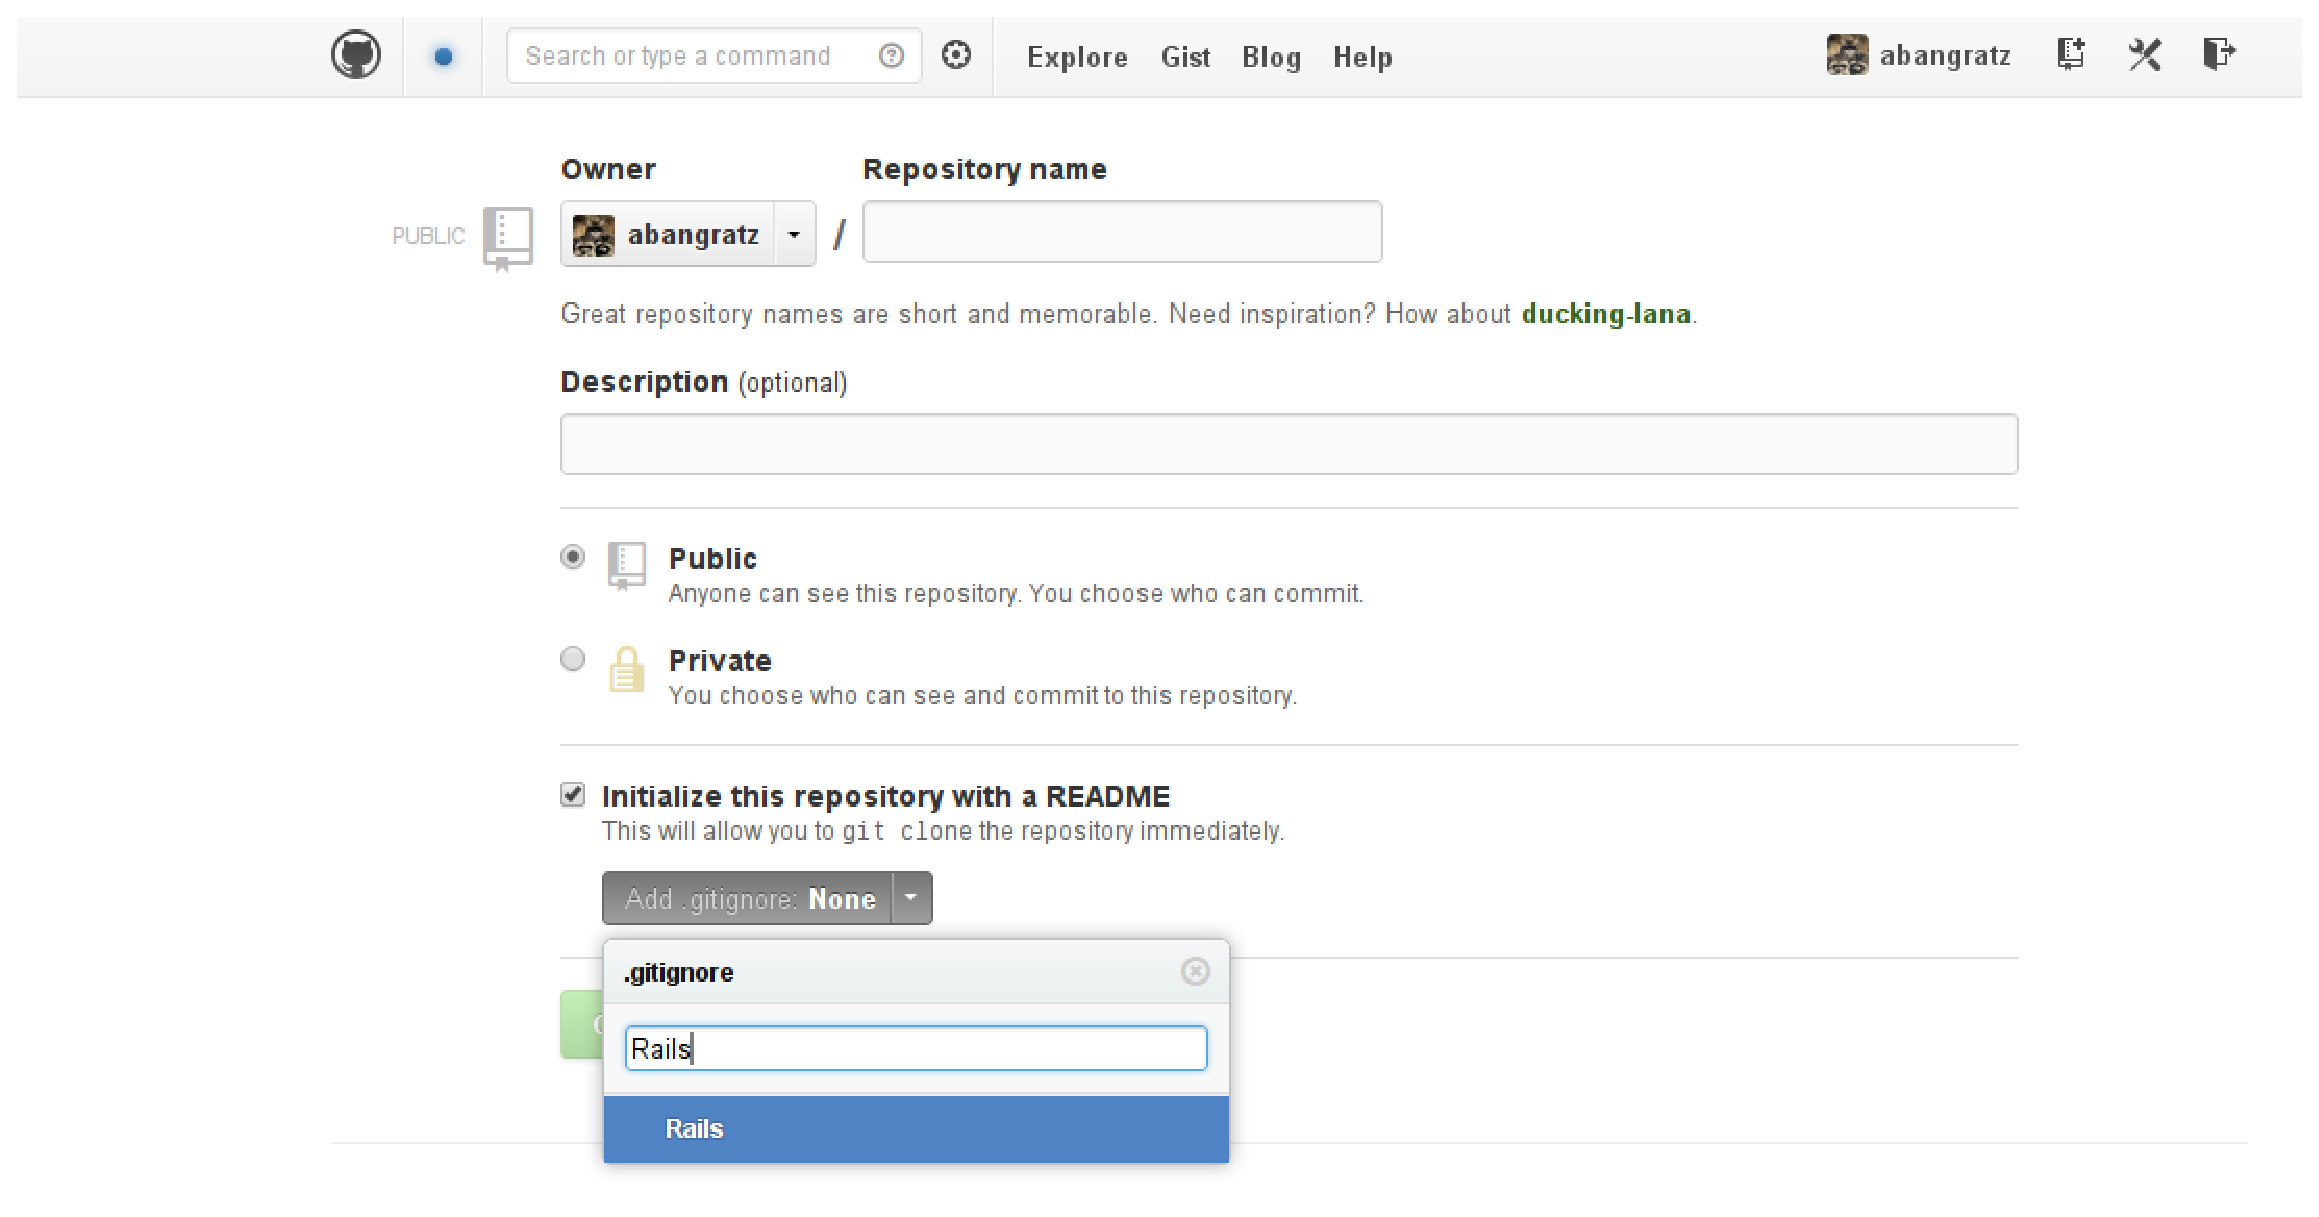
\includegraphics[scale=0.35]{rails_github_new.eps}
\end{slide}
\begin{slide}{.gitignore}
	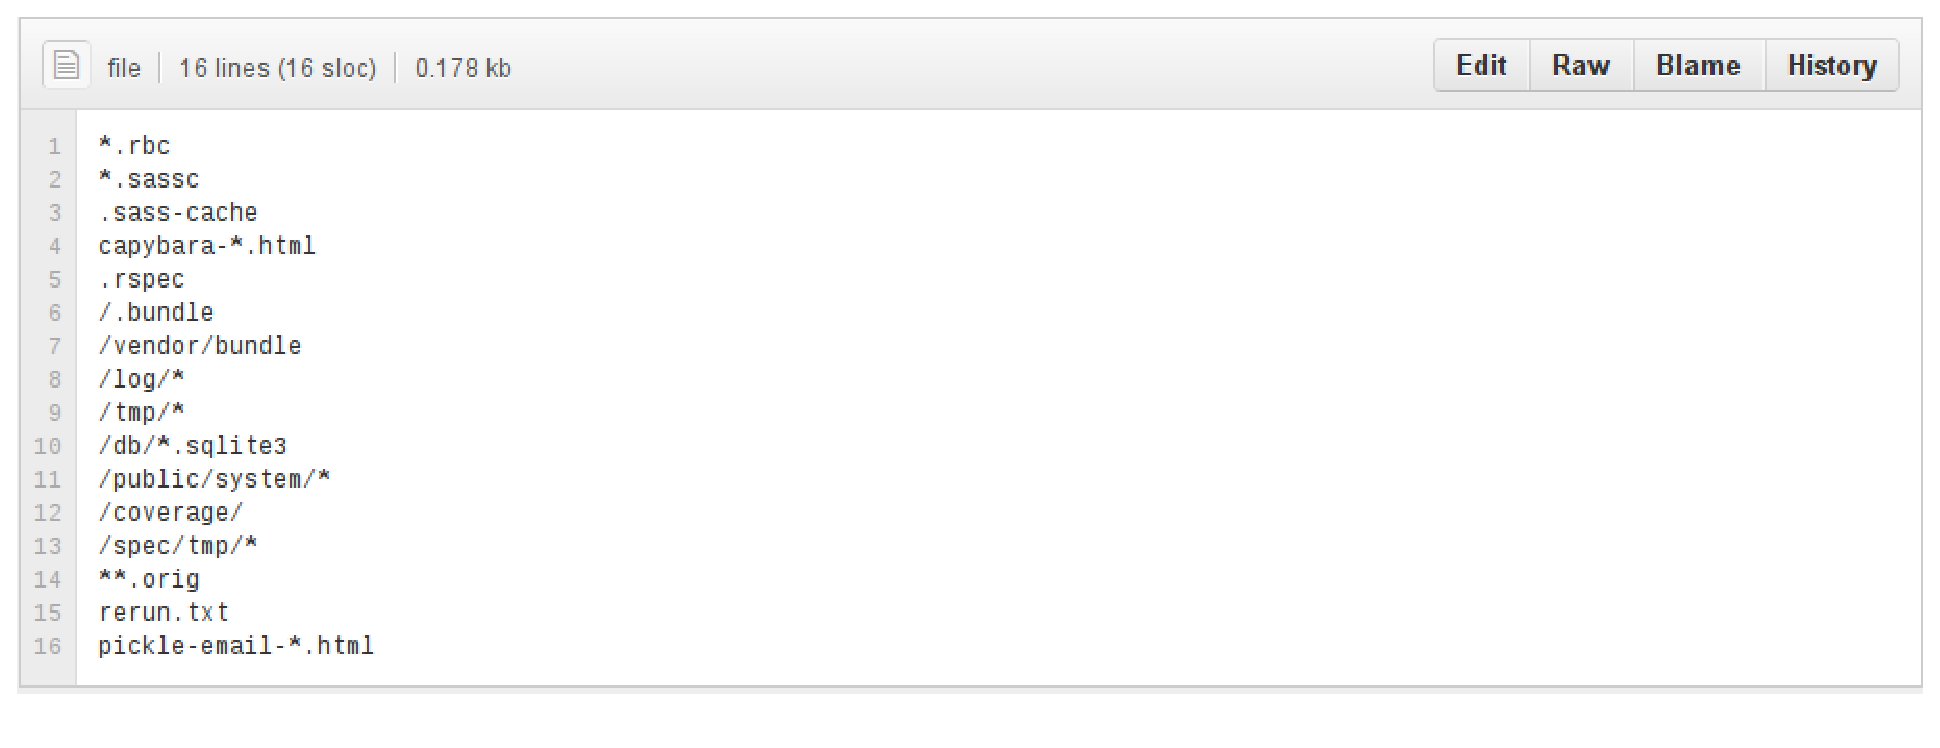
\includegraphics[scale=0.35]{rails_gitignore.eps}
\end{slide}
\section{Workflow}
\begin{slide}{Init, Fork and Clone}
	\includegraphics[scale=0.25]{forktocat.eps}
\end{slide}
\begin{note}{Init, Fork, Clone}
	\begin{itemize}
		\item[Init] is preparing a new repository locally.
		\item[Fork] is making a copy of a repository on GitHub that links back to the original.
		\item[Clone] is making a local copy of a remote repository.
	\end{itemize}
\end{note}
\begin{slide}{Commit, Pull and Push}
	\includegraphics[scale=0.25]{setuptocat.eps}
\end{slide}
\begin{note}{The Standard Workflow}
	\begin{itemize}
		\item[Add] is adding a file to be committed (rm removes).
		\item[Commit] is preparing a changeset to be created (pending message).
		\item[Pull] is fetching and synchronizing all changes from remote to local (conflicts may be merged or have
			to be resolved!).
		\item[Push] is pushing the outstanding changesets from local to remote (if this fails, pull first and
			resolve conflicts).
	\end{itemize}
\end{note}
\begin{slide}{Fork, Branch and Pull Request}
	\includegraphics[scale=0.25]{socialite.eps}
\end{slide}
\begin{note}{Why the hard work?}
	\begin{itemize}
		\item Creating \textit{topic branches} helps organizing work on different features. It also helps to
			coordinate a team (split personality notwithstanding).
		\item \textit{Forking} is a way to work on a project you cannot contribute directly and lets the original owner
			decide if they want to integrate your changes into their repository.
		\item \textit{Pull requests} are the most simple way to package changes and comments to be integrated from a fork into the
			original repository (caveat: git and GitHub pull requests are more than subtly different animals).
	\end{itemize}
\end{note}
\section{Tips and Tricks}
\begin{slide}{Collaboration and Comments}
	\includegraphics[scale=0.2]{collabocats.eps}
\end{slide}
\begin{note}{Collaboration and Comments}
	\begin{itemize}
		\item Use the \textit{Admin} menu for assigning teams and collaborators to a repository.
		\item Comment files and pull requests via the GitHub web interface - only in commits!
		\item Use \url{@user}--Notation inline to notify collaborators and friends directly. (e.g. \url{@abangratz} -
			autocompletion included).
		\item Use issues to report bugs - and issue numbers to reference them in comments and commit messages.
		\item Keep commit messages short and clean.
		\item Commit small changesets - often is better.
		\item Use Gist to share and collaborate on small snippets.
		\item Don't be afraid: you can't really destroy anything. Even collaborating on rails/rails is no big issue.
	\end{itemize}
\end{note}
\begin{note}{Socializing}
	\begin{itemize}
		\item Following
		\item Wall
		\item Collaboration
		\item Graphs
		\item Activity
		\item Profile / Team/Company membership
		\item Notifications
		\item Starring
	\end{itemize}
\end{note}
\section[tocsection=hidden,slide=false]{End}
\begin{emptyslide}{}
	\centering
	
\includegraphics[scale=0.2]{octobiwan_source.eps}
\end{emptyslide}
\end{document}
